\subsection{主案例实跑：从首期积水初报到核查简报}
三轮请求从同一工作台提交，Pi 通过 Responses 调用模型（服务名 \code{gpt-6.1-sol}）。用户指定日期和任务目标，没有指定分割算法。图~\ref{fig:karla-decisions} 追踪从请求到结果的三次判断，表~\ref{tab:karla-turns} 用实际参数和文件数核对每次判断。完整请求、选法理由、函数参数和工具返回保存在 \code{karla.json}。

\begin{figure}[H]
\centering
\begin{tikzpicture}[x=1mm,y=1mm,
  input/.style={text width=34mm,minimum height=18mm,inner sep=2.2mm,align=left,
    draw=black!17,fill=black!2,line width=.5pt,font=\small},
  decision/.style={input,text width=49mm,draw=ucasblue!34,fill=ucasblue!7},
  output/.style={input,text width=42mm,draw=agentteal!36,fill=agentteal!5},
  link/.style={-{Latex[length=1.7mm]},draw=ucasblue!63,line width=.58pt},
  head/.style={font=\small\bfseries,text=reportmuted}]
  \node[head] at (0,0) {用户这轮要什么};
  \node[head] at (49,0) {Pi 看了什么、决定什么};
  \node[head] at (102,0) {工具算出或保留什么};
  \node[input] (u1) at (0,-16) {\textbf{1\enspace 截至 18 日初报}\\从可用像元提取候选};
  \node[decision] (d1) at (49,-16) {同轨 7、双极化、共同有效率 100\%\\\textbf{选择 SAR 变化法}};
  \node[output] (p1) at (102,-16) {在线下载、分割并发布\\\textbf{71.19 \km 雷达候选}};
  \node[input] (u2) at (0,-48) {\textbf{2\enspace 更新至 19 日}\\新观测与旧图对照};
  \node[decision] (d2) at (49,-48) {光学共同有效率 96.45\%\\\textbf{改用 MNDWI，引用两期掩膜}};
  \node[output] (p2) at (102,-48) {保留雷达图；新增光学图和四类证据对照};
  \node[input] (u3) at (0,-80) {\textbf{3\enspace 发布核查清单}\\分别算全窗与北部};
  \node[decision] (d3) at (49,-80) {同一套观测、只改变范围\\\textbf{复用对照 ID，调用两次叠加}};
  \node[output] (p3) at (102,-80) {两套独立地图、耕地和路段清单；\textbf{未重下或重分割}};
  \foreach \i in {1,2,3}{
    \draw[link] (u\i.east) -- (d\i.west);
    \draw[link] (d\i.east) -- (p\i.west);
  }
  \draw[link,dashed,draw=agentteal] (p1.south) -- ++(0,-6.3)
    -- node[above,font=\scriptsize,text=agentteal,inner sep=1pt]{复用雷达掩膜} ++(-53,0) -- (d2.north);
  \draw[link,dashed,draw=agentteal] (p2.south) -- ++(0,-6.3)
    -- node[above,font=\scriptsize,text=agentteal,inner sep=1pt]{复用证据对照} ++(-53,0) -- (d3.north);
\end{tikzpicture}
\caption{从三轮真实工具日志整理的决策图。实线是本轮请求和产出，绿色虚线是跨轮复用。第二轮更换观测与算法；第三轮仅改变分析范围。两类判断分别落到不同的工具参数，而不是改变回复措辞。}
\label{fig:karla-decisions}
\end{figure}

\begin{figure}[htbp]
\centering
\begin{tabular}{@{}p{.476\linewidth}@{\hspace{.04\linewidth}}p{.476\linewidth}@{}}
\sffamily\small\bfseries a\enspace 更新观测与证据对照 &
\sffamily\small\bfseries b\enspace 复用证据开展分区核查\\[3pt]
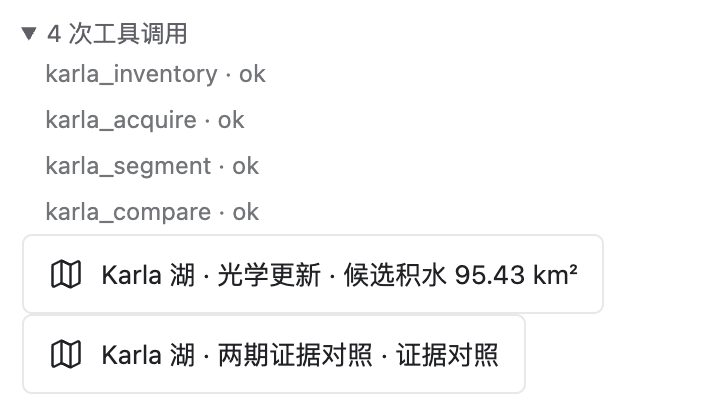
\includegraphics[width=\linewidth]{figures/karla-optical-update.png} &

\includegraphics[width=\linewidth]{figures/karla-reuse-exposure.png}
\end{tabular}
\caption{FloodLab 工作台中的真实执行截图，裁切自同一会话的第二、三轮回复，未改动内容。a：下载、分割和对照均有成功记录，下方是光学更新图与两期对照图；b：只有读取已有资料及两次分区核查的记录，各自对应一个成果入口。}
\label{fig:karla-workbench-traces}
\end{figure}


\begin{table}[htbp]
\centering
\caption{三轮工具调用的决策参数与产物。完整记录见成果包。}
\label{tab:karla-turns}
\small
\begin{tabularx}{\linewidth}{@{}>{\raggedright\arraybackslash}p{22mm}>{\raggedright\arraybackslash}p{60mm}>{\raggedright\arraybackslash}X@{}}
\toprule
轮次 & 模型调用的关键参数 & 工具结果\\
\midrule
18 日初报（3 次） & \code{sensor=sar}；\code{algorithm=sar_change}。选法理由附同轨 7 和实际覆盖。 & 在线下载；候选 71.1892 \km，333 个矢量斑块。\\
19 日更新（4 次） & \code{sensor=optical}；\code{algorithm=optical_mndwi}；对照函数收到雷达和光学两个掩膜 ID。 & 在线下载；光学候选 95.4260 \km、126 个斑块；另有一张对照图。\\
分区核查（3 次） & 两次传入同一 \code{comparison_id}，分别设 \code{scope=study}、\code{scope=north}。 & 两套清单，159 和 103 个路段片段；下载、分割调用各为 0。\\
\bottomrule
\end{tabularx}
\end{table}

\begin{figure}[H]
\centering
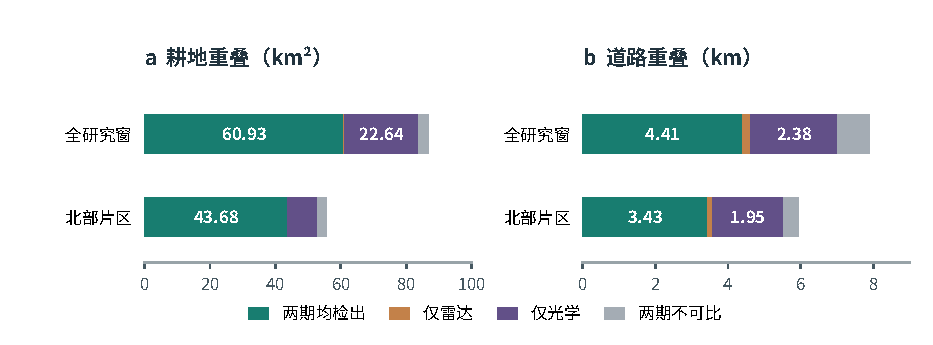
\includegraphics[width=\linewidth]{figures/karla-screening.pdf}
\caption{全研究窗和北部片区的暴露核查。a：耕地重叠面积；b：所选 OSM 道路中心线重叠长度。紫色为单期光学线索，灰色为两期不可比。全窗包含北部片区。}
\label{fig:karla-screening}
\end{figure}

\paragraph{新增观测改变了什么。}
图~\ref{fig:karla-compare} 显示两期均检出 66.9064 \km，仅雷达 1.1196 \km、仅光学 28.5196 \km，另有 23.2508 \km 不可跨期比较。其中 3.1632 \km 在初报中有雷达候选，但缺少可用的光学判读，归入不可比。共同可判读区内，雷达初报涉及 68.0260 \km；光学更新将其中 66.9064 \km 标为两期均检出，并补充只由光学发现的核查线索。与官方同日轮廓的交并比分别为 0.736 和 0.935，反映与基于同批观测制作的参考图之间的空间一致性。

\paragraph{核查名单怎样变化。}
图~\ref{fig:karla-screening} 量化证据更新对清单的影响：全窗仅光学的部分对应额外 22.64 \km 耕地和 2.38 km 道路线索，仍需按单期证据核查。缩小到北部后，约 0.41 km 所选道路处于两期不可比区，应保留为未知。表~\ref{tab:karla-shortlist} 将这种区别落实到路段：两期均检出可优先核对通行记录，单期线索应复判原片，不可比则需补观测。完整清单可通过对应专题图（图~\ref{fig:karla-exposure}）和 CSV 定位；重叠不等于灾时道路封闭。

\begin{table}[H]
\centering
\caption{北部核查清单摘录，按证据类别各取第一条。编号和坐标可在清单及 QGIS 中定位。}
\label{tab:karla-shortlist}
\small
\begin{tabularx}{\linewidth}{@{}p{23mm}p{26mm}r>{\raggedright\arraybackslash}p{36mm}>{\raggedright\arraybackslash}X@{}}
\toprule
证据类别 & OSM way ID & 米 & 中点经纬度（东、北） & 建议核查\\
\midrule
两期均检出 & 538784698 & 865.50 & 22.685619, 39.588435 & 优先核对通行记录\\
仅光学 & 425625350 & 511.06 & 22.720085, 39.555781 & 查影像原片与日期\\
仅雷达 & 538784696 & 24.08 & 22.692878, 39.591697 & 核对该段散射条件\\
两期不可比 & 169155643 & 387.18 & 22.715405, 39.595497 & 补充观测，不作判断\\
\bottomrule
\end{tabularx}
\end{table}

\paragraph{成果验收。}
独立程序核对了像元与矢量面积、证据分类和路段长度，五份 QGIS 工程均通过打开检查。

\clearpage
\begin{landscape}
\thispagestyle{empty}
\noindent\begin{minipage}[c][148mm][c]{\linewidth}
\centering
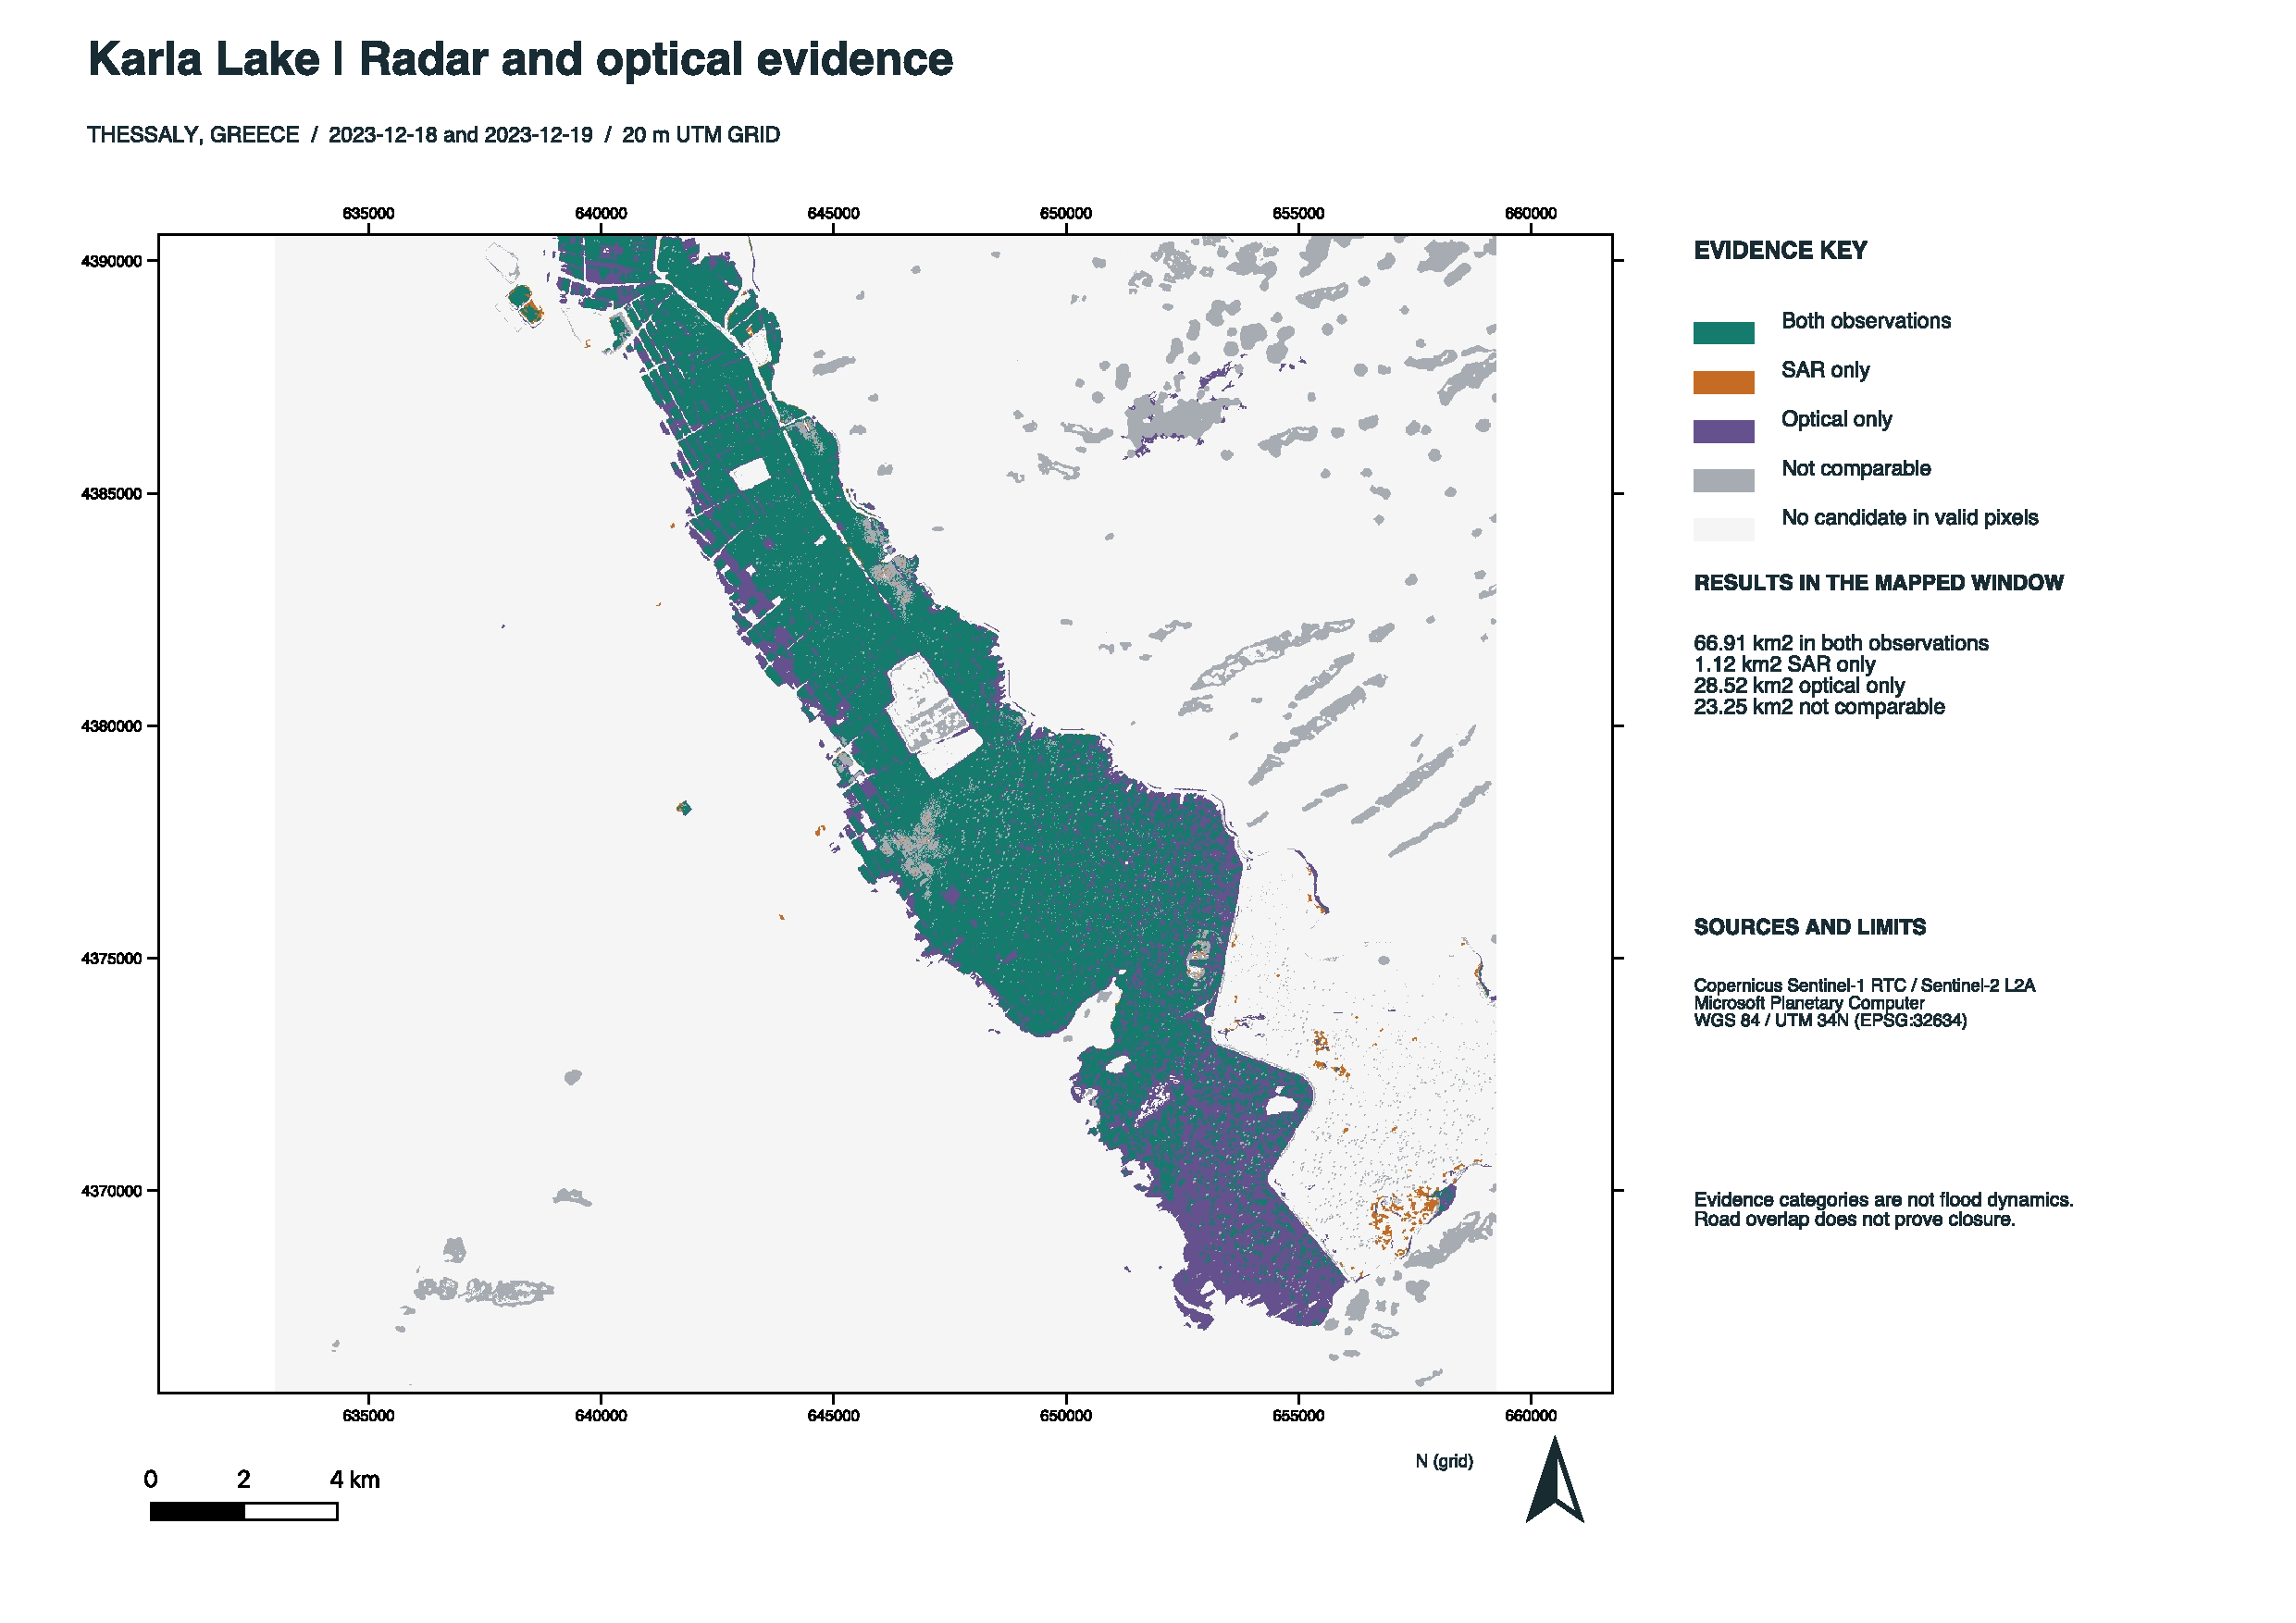
\includegraphics[width=\linewidth,height=136mm,keepaspectratio]{evidence/karla/outputs/comparison-ce8daf32d0/map.pdf}
\captionsetup{hypcap=false}
\captionof{figure}{Karla 湖两期遥感证据对照。灰色表示两期不可比的像元。}
\label{fig:karla-compare}
\end{minipage}\par
\noindent\hfill{\sffamily\small\color{reportmuted}\thepage}\hfill\mbox{}
\end{landscape}

\begin{landscape}
\thispagestyle{empty}
\noindent\begin{minipage}[c][148mm][c]{\linewidth}
\centering
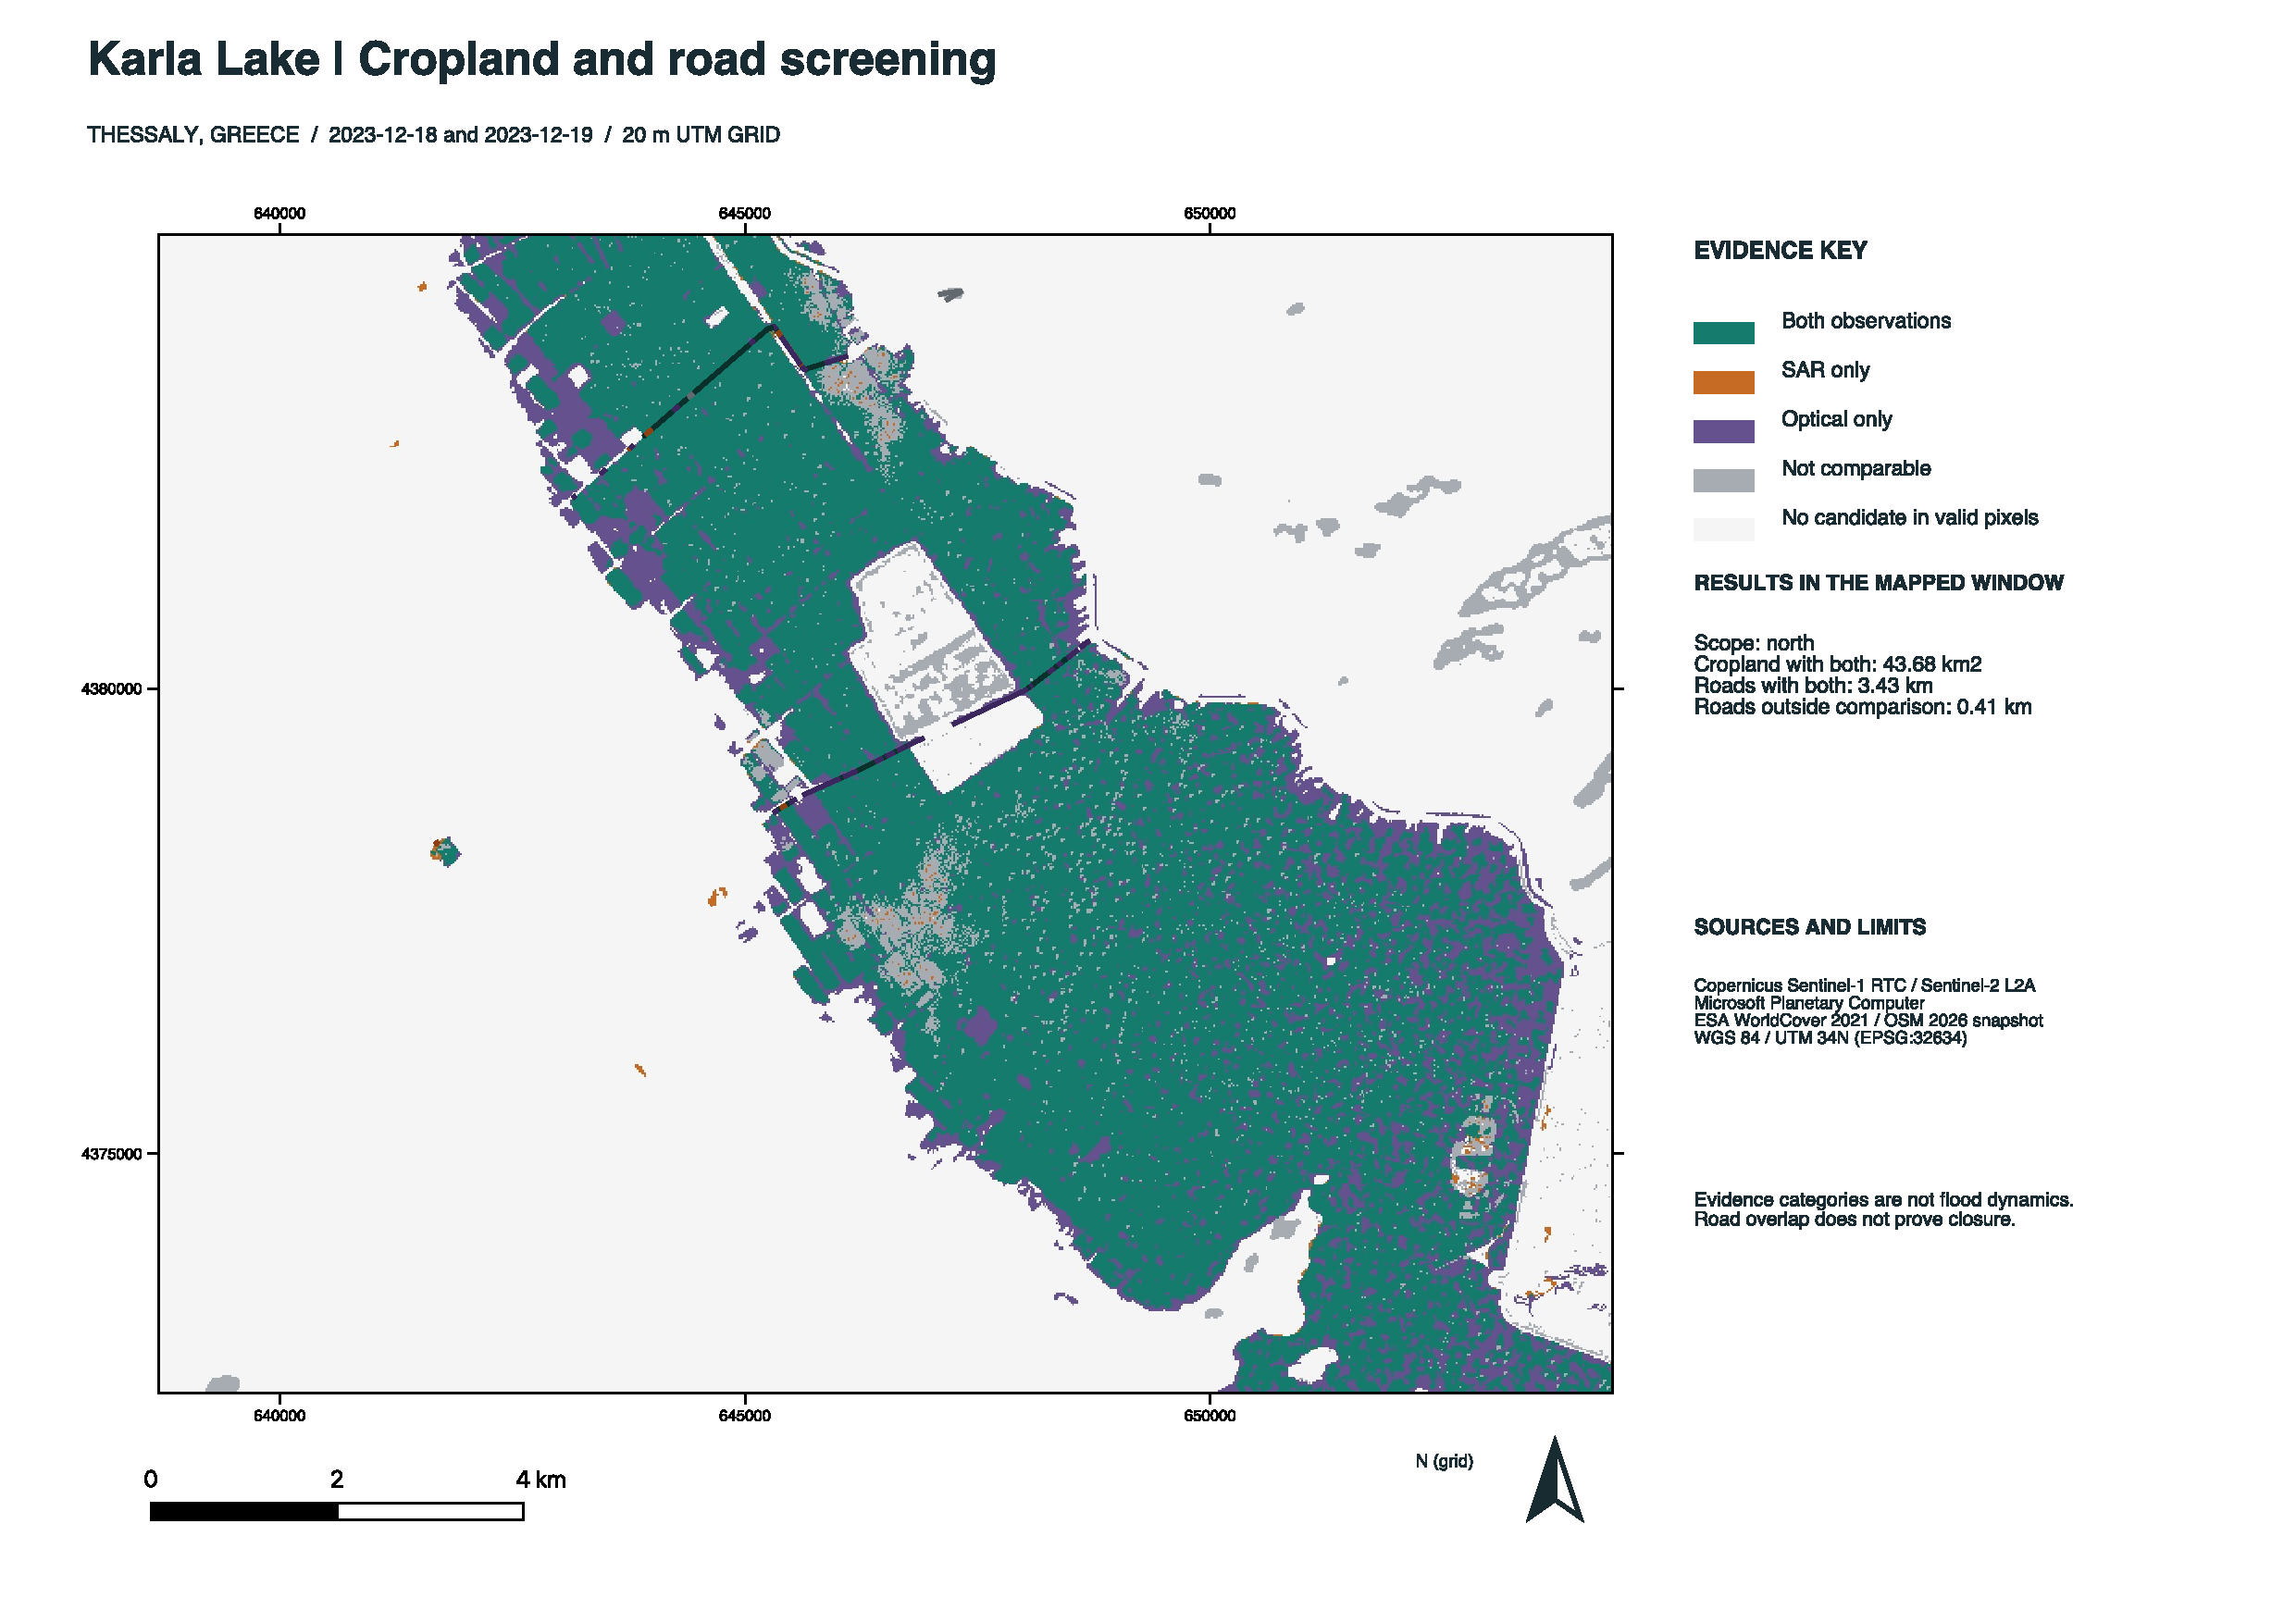
\includegraphics[width=\linewidth,height=136mm,keepaspectratio]{evidence/karla/outputs/exposure-4fa28e86a4/map.pdf}
\captionsetup{hypcap=false}
\captionof{figure}{Karla 湖北部片区核查图。配套清单提供路段中点、重叠长度及证据类别。道路使用 2026 年 OSM 快照。}
\label{fig:karla-exposure}
\end{minipage}\par
\noindent\hfill{\sffamily\small\color{reportmuted}\thepage}\hfill\mbox{}
\end{landscape}
